\documentclass{cmspaper}
\usepackage{lineno}
\usepackage{amsfonts,amsmath,amssymb}
\usepackage[dvips]{graphicx}
\usepackage{bm}
\usepackage{multirow}
\usepackage{subfigure}  % use for side-by-side figures
%\usepackage[a4paper]{hyperref}

\def\etmiss{\big\slash\hspace{-1.6ex}{E_\text{T}}}
\def\etmissB{\big\slash\hspace{-1.6ex}{\boldsymbol{E}_\text{T}}}
\def\exmiss{\big\slash\hspace{-1.6ex}{E_{x}}}
\def\eymiss{\big\slash\hspace{-1.6ex}{E_{y}}}
\def\sumet{\sum{E_\text{T}}}
\def\sumetB{\sum{\boldsymbol{E}_\text{T}}}

\begin{document}
\begin{linenumbers}


\begin{titlepage}

  % select one of the following and type in the proper number:

%  \cmsnote{2010/001}
  \internalnote{2010/XXX}
%  \conferencereport{2005/000}
%  \cmsan{2010/029}
%  \cmsdtnote{2005/000}
%  \cmspas{2005/000}
   \date{\today}

  \title{Results of visual scan of high $\etmiss$ events in 7 TeV pp collision data}

  \begin{Authlist}
    %A.~Apresyan
    %\Instfoot{caltech}{California Institute of Technology, Pasadena, CA, USA}
    H.~Liu
    \Instfoot{bayu}{Baylor University, Waco, TX, USA}
    D.~Ferencek, F.~Santanastasio %\Aref{a}
    \Instfoot{umd}{University of Maryland, College Park, MD, USA}   
  \end{Authlist}

% if needed, use the following:
%\collaboration{CMS collaboration}

%\Anotfoot{a}{Also at \textit{California Institute of Technology, Pasadena, CA, USA}}

  \begin{abstract}    
   We present the results of a visual scan of high $\etmiss$ events 
   (tc$\etmiss>60$~GeV OR pf$\etmiss>60$~GeV)
   in an inclusive sample of XX~nb$^{-1}$ of 7 TeV pp collision data, 
   after applying the official noise clean-up available in CMSSW\_3\_7\_0\_patch2. 
   The scan is performed separately for events with tc$\etmiss>60$~GeV and pf$\etmiss>60$~GeV
   since the noise clean-up is implemented differently in the two $\etmiss$ algorithms.
   The CMS software {\it Fireworks} has been used to produce the event displays. 
   The high $\etmiss$ events have been visually inspected and classified in different 
   cathegories. The results of this scan can provide hints to further improve the noise 
   cleaning and to identify possible problems and inconsistencies in the algorithms employed 
   in CMS for the $\etmiss$ reconstruction.
  \end{abstract} 

% if needed, use the following:
%\conference{Presented at {\it Physics Rumours}, Coconut Island, April 1, 2005}
%\submitted{Submitted to {\it Physics Rumours}}
%\note{Preliminary version}
  
\end{titlepage}

\setcounter{page}{2}%JPP

\tableofcontents

\clearpage

\section{Introduction}

Commissioning studies performed with test beams, cosmic runs and 
early 0.9~TeV, 2.36~TeV and 7~TeV pp 
collision data have identified several sources of anomalous noise 
(i.e. noise not produce solely from expected fluctuations in the electronics)
in the calorimeters of the CMS experiment:
\begin{itemize}
\item {\it ECAL barrel spikes} - Energy deposits in individual channels 
affected by the noise are cleaned using both topological and 
timing information of the reconstructed hits. Noise correlated with collisions. 
More details are available at XXX.
\item {\it HF PMT hits} - Energy deposits in individual channels 
affected by the noise are cleaned using both topological and 
timing information of the reconstructed hits. Noise correlated with collisions. 
More details are available at XXX.
\item {\it HPB/RBX noise in HCAL barrel and endcaps} - Events with identified 
HPD/RBX noise are removed from the analysis using a filter based on both topological 
and timing information of the reconstructed energy deposits. Noise not correlated 
with collision. More details are available at XXX.
\end{itemize}
In addition, machine-induced background, in the form of 
beam halo [XXX] and beam scraping events [XXX], have been observed. 

The overlap of either anomalous noise or machine-induced background 
with a pp collision event produces an unbalance in 
the reconstructed missing transverse energy in the event, which can produce 
large tails in the $\etmiss$ distribution. 

In this note, we present the results of a visual scan of high $\etmiss$ events 
($>45$~GeV) %(Calo$\etmiss>45$~GeV OR tc$\etmiss>45$~GeV OR pf$\etmiss>45$~GeV)
in a sample %of 12~nb$^{-1}$ 
of 7 TeV pp collision data, after applying the 
%official 
noise clean-up developed by joint effort of several groups in the CMS collaboration, 
and described in Section~\ref{sec:EventSelection}. 
The CMS software {\it Fireworks} [XXX] has been used to produce the event displays. 
The high $\etmiss$ events have been visually inspected and classified in different 
cathegories. The resuls of this scan can be used as a starting point to further improve 
the noise cleaning algorithms and to identify possible problems and inconsistencies 
in the three algorithms employed in CMS for the $\etmiss$ reconstruction.


\section{Datasample, Event Selection, and Noise Cleaning} \label{sec:EventSelection}

{\bf Dataset and CMSSW release:}
\begin{itemize}
\item dataset: /MinimumBias/Commissioning10-GOODCOLL-Jun9thSkim\_v1/RECO
\item CMSSW release: CMSSW\_3\_7\_0\_patch2
\end{itemize}

{\bf Event selection:}
\begin{itemize}
\item Physics declared bit
\item BPTX bit 0
\item Removal of beam scraping events
\item Good primary vertex
\item Good Run/LS selection. JSON file: Cert\_132440-136119\_7TeV\_May27thReReco\_Collisions10\_JSON.txt  
\end{itemize}
More details at [XXX].

{\bf Noise cleaning}

Noise cleaning/event filter for calotower-based $\etmiss$ algorithms (Calo$\etmiss$ and tc$\etmiss$):
\begin{itemize}
\item ECAL barrel spikes (reject RecHits): topology (kWeird flag = swiss cross variable) + timing (kOutOfTime flag) [XXX];
\item HF PMT hits (reject Rechits): topology (HFLongShort flag = PET+S9/S1) + pulse shape (HFDigiTime flag) [XXX];
\item HPD/RBX noise in HBHE (reject events): combination of pulse shape and topological variables [XXX].
\end{itemize}

Noise cleaning (reject RecHits) for pf$\etmiss$ is described at [XXX]. Timing and topology are used to reject RecHits 
affected by ECAL and HF noise. Topology only is used to reject rechits affected by HBHE noise. No events are rejected.

NOTE: The HPD/RBX noise filter is applied for both the tc$\etmiss$ and pf$\etmiss$ analysis presented in this note, 
in order to have the same number of events passing the selection.

%Figure~\ref{fig:calomet} shows the cleaned Calo$\etmiss$ distribution for $\approx 19.6$~M events 
%passing the event selection described above.
%\begin{figure}[h]
% \centering
% \begin{tabular}{ll}
%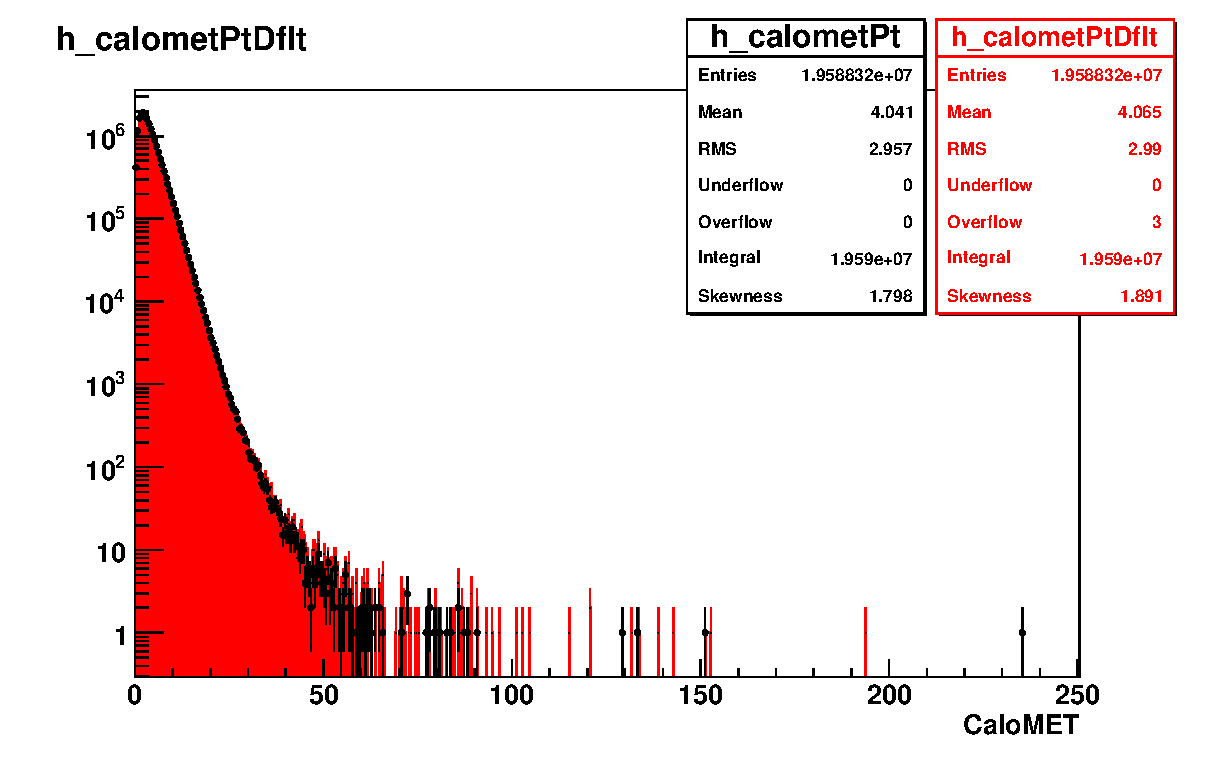
\includegraphics[width=0.7\textwidth]{fig/calomet.eps} 
% \end{tabular}
%\caption{Calo$\etmiss$ distribution of 7 TeV collision data after applying the event selection described
%in this section. Red filled histogram is obtained using the $\etmiss$ value coming from default CMS reconstruction 
%in CMSSW\_358p3. The black dotted histogram is the $\etmiss$ after applying the full noise cleaning 
%procedure described in this section.}
%\label{fig:calomet}
%\end{figure}
\section{Scan of high $\etmiss$ events}

Two high $\etmiss$ skims have been produced and stored in the directory \\ 
SKIMDIR = XXXXX :
\begin{itemize}
\item tc$\etmiss$ skim: tc$\etmiss>60$~GeV \\ 
Root file in RECO format at: \\ SKIMDIR/YYYY
\item pf$\etmiss$ skim: pf$\etmiss>60$~GeV \\
Root file in RECO format at: \\ SKIMDIR/YYYY
\end{itemize}

A visual scan of these events have been performed using the CMS event display
software ``Fireworks''. We decided to compare tc$\etmiss$ and pf$\etmiss$ 
tails, since they both uses tracker information to correct the $\etmiss$ 
measurement, while we excluded raw Calo$\etmiss$ algorithm from the analysis, which only relies 
on calorimeter information (and therefore provides a lower $\etmiss$ resolution).

It should pointed out that the results of a visual scan 
are always subject to a personal judgment. 
Nevertheless, they should provide, with good approximation, a realistic 
picture of the events populating the $\etmiss$ tails after applying 
the current noise clean-up. 

The result of the scan for tc$\etmiss$ skim and pf$\etmiss$ skim are summarized 
in the Tables~\ref{tab:tcMETskim} and ~\ref{tab:pfMETskim}, respectively.

% tcMET skim
\begin{table}[htbp]
  \begin{center}
    \begin{tabular}{|c|c|c|c|}
      \hline
      \multicolumn{2}{|c|}{Category} & Number of events  & Comments   \\ 
      \hline\hline
      \multicolumn{2}{|c|}{\bf ECAL} & \bf{25}      &  \\
      \hline
      EB & spike at EB-EE boundary & 23 & all removed by Particle-Flow cleaning \\     
      EB & spike & 1 & removed by Particle-Flow cleaning \\     
      EE & spike & 1 & removed by Particle-Flow cleaning \\     
      \hline    
      \multicolumn{2}{|c|}{\bf HCAL} & \bf{45}      &  \\
      \hline
      HF & multi-PMT-hits or phi-strip events & 12 & 5 cleaned by Particle-Flow cleaning \\           
      HF & double-PMT-hits & 23 & 18 cleaned by Particle-Flow cleaning \\           
      HF & PMT hit embedded in a jet & 3 & not cleaned by Particle-Flow cleaning \\           
      HB & IonFeedback/HPD/RBX noise & 6 & low-multipl. noise, not cleaned by PF\\           
      HE & IonFeedback/HPD/RBX noise & 1 & low-multipl. noise, not cleaned by PF \\           
      \hline    
      \multicolumn{2}{|c|}{\bf PHYSICS} & \bf{36}      &  \\
      \hline
      Physics & 1 jet & 1 & large pf$\etmiss$ as well \\
      Physics & 2 jets & 10 & 6 of them have pf$\etmiss$ $<$ OR $<<$ than tc$\etmiss$ \\
      Physics & 3 jets & 12 & 5 of them have pf$\etmiss$ $<$ OR $<<$ than tc$\etmiss$ \\
      Physics & 4 jets & 9 & 4 of them have pf$\etmiss$ $<$ OR $<<$ than tc$\etmiss$ \\
      Physics & 5 jets & 2 & 1 of them has pf$\etmiss$~$\approx$1/2$\times$~tc$\etmiss$\\
      Physics & 6 jets & 2 & both have pf$\etmiss$~$\approx$1/2$\times$~tc$\etmiss$\\
      \hline
      \multicolumn{2}{|c|}{\bf OTHERS} & \bf{1}      &  \\
      \hline          
      Others & HB activity + muon & 1 & large pf$\etmiss$ as well \\
      \hline          
      \multicolumn{2}{|c|}{\bf TOTAL} & \bf{107}      &  \\
      \hline
    \end{tabular}
    \caption{Results of visual scan of events with tc$\etmiss>60$~GeV.}        
    \label{tab:tcMETskim}
  \end{center}
\end{table}
%
% pfMET skim
%
\begin{table}[htbp]
  \begin{center}
    \begin{tabular}{|c|c|c|c|}
      \hline
      \multicolumn{2}{|c|}{Category} & Number of events  & Comments   \\ 
      \hline\hline
      \multicolumn{2}{|c|}{\bf ECAL} & \bf{0}      &  \\
      \hline    
      \multicolumn{2}{|c|}{\bf HCAL} & \bf{19}      &  \\
      \hline
      HF & multi-PMT-hits or phi-strip events & 4 & large tc$\etmiss$ as well \\           
      HF & double-PMT-hits & 4 & large tc$\etmiss$ as well \\           
      HF & PMT hit embedded in a jet & 3 & large tc$\etmiss$ as well \\           
      HB & IonFeedback/HPD/RBX noise & 7 & low-multipl. noise, large tc$\etmiss$ as well \\           
      HE & IonFeedback/HPD/RBX noise & 1 & low-multipl. noise, large tc$\etmiss$ as well \\           
      \hline    
      \multicolumn{2}{|c|}{\bf PHYSICS} & \bf{18}      &  \\
      \hline
      Physics & 1 jet & 1 & large tc$\etmiss$ as well \\
      Physics & 2 jets & 5 & large tc$\etmiss$ as well \\
      Physics & 3 jets & 6 & large tc$\etmiss$ as well \\
      Physics & 4 jets & 3 & large tc$\etmiss$ as well \\
      Physics & 5 jets & 1 & large tc$\etmiss$ as well\\
      Physics & 6 jets & 1 & pf$\etmiss$~$\approx$2$\times$~tc$\etmiss$\\
      Physics & jet + muon & 1 & large tc$\etmiss$ as well \\ 
      \hline
      \multicolumn{2}{|c|}{\bf OTHERS} & \bf{6}      &  \\
      \hline          
      Others & large muon-induced pfMET & 5 & very small calo$\etmiss$/tc$\etmiss$ \\ 
      Others & HB activity + muon & 1 & large tc$\etmiss$ as well \\
      \hline          
      \multicolumn{2}{|c|}{\bf TOTAL} & \bf{43}      &  \\
      \hline
    \end{tabular}
    \caption{Results of visual scan of events with pf$\etmiss>60$~GeV.}    
    \label{tab:pfMETskim}
  \end{center}
\end{table}

\section{Description and event displays of high $\etmiss$ events}

\subsection{EB, spike at EB-EE boundary}
We see EB spikes occurring at the boundary between ECAL barrel and endcaps.

The ECAL spikes topological cuts employed in the calotower cleaning for Calo$\etmiss$ and tc$\etmiss$ 
are not currently applied to identify ``spikes'' candidates occuring at the boundary between ECAL barrel and endcaps. 
Most of such events should be removed by the timing cuts. Nevertheless, some of them still survives 
after the noise clean-up, as the event shown in Figure~\ref{fig:EBspikeAtBorder}.

Such EB spikes are instead all cleaned by PF cleaning, which applies relaxed topological cuts also at the EB-EE boundary.
%
\begin{figure}[h]
 \centering
% \begin{tabular}{ll}
   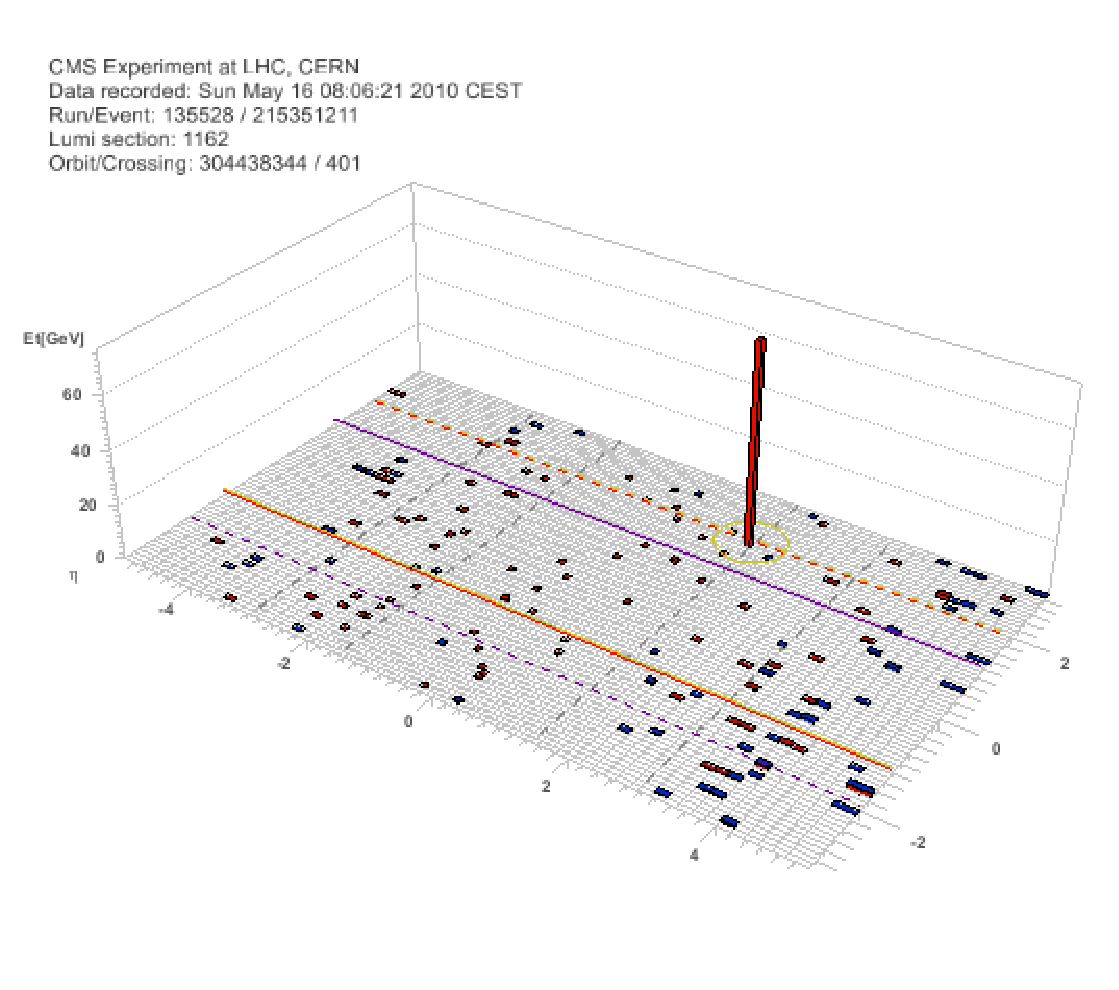
\includegraphics[width=0.47\textwidth]{fig/EBspikeAtBorder.eps} 
% \end{tabular}
\caption{Example of ``EB spike at EB-EE boundary'' event}
\label{fig:EBspikeAtBorder}
\end{figure}

\subsection{EB, EE spikes}
We see one event with an isolated spike in EB (Figure~\ref{fig:EBEEspike}, left plot) 
and one event with an isolated spike in EE (Figure~\ref{fig:EBEEspike}, right plot), both far from the EB-EE boundaries.

Calotower-based cleaning for spikes is not applied in EE (since the spikes has been observed and understood 
as due to interaction of particles in APD, which are mounted only in the barrel). 
The case of EB spike not cleaned should be investigated.

Both events are cleaned by PF (which applies spike cleaning also in EE).
%
\begin{figure}[h]
 \centering
 \begin{tabular}{ll}
   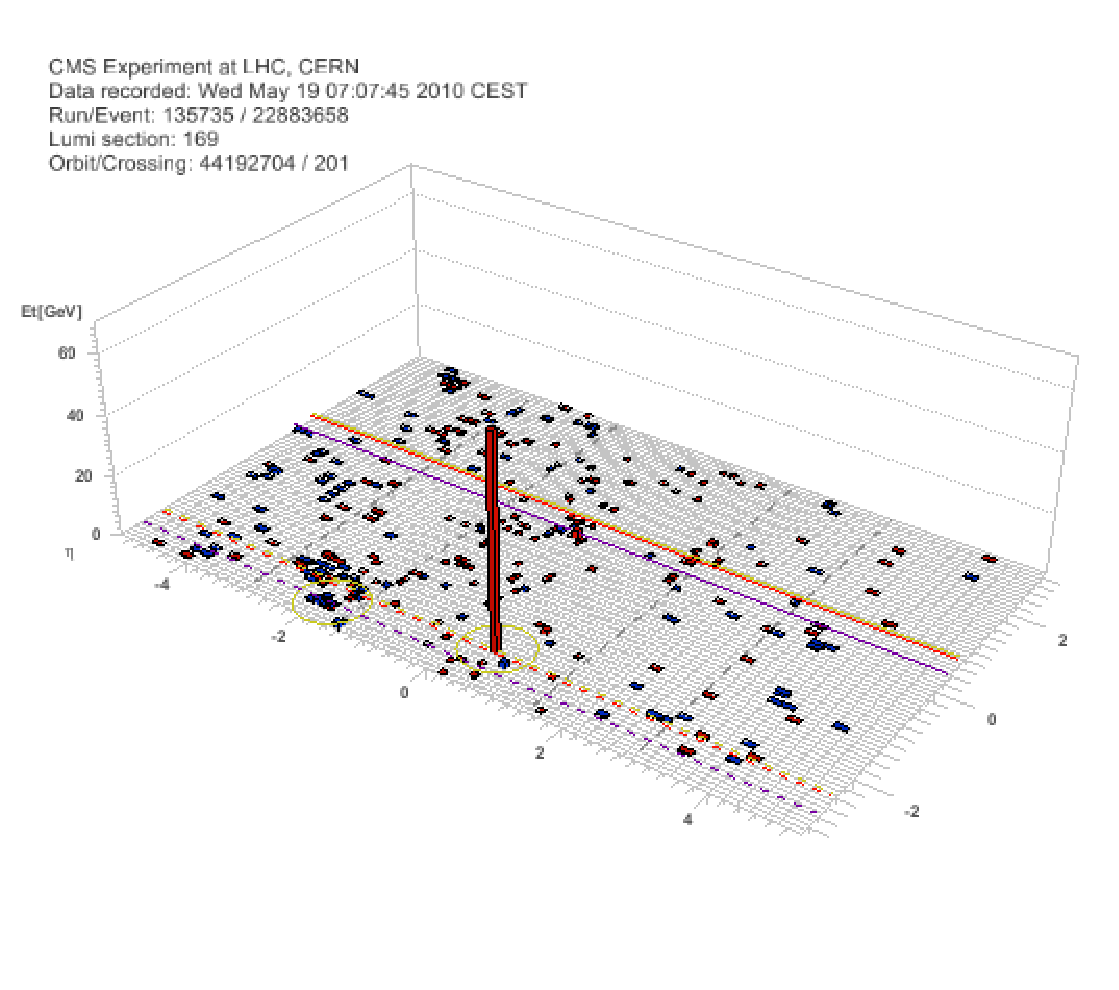
\includegraphics[width=0.47\textwidth]{fig/EBspike.eps} &
   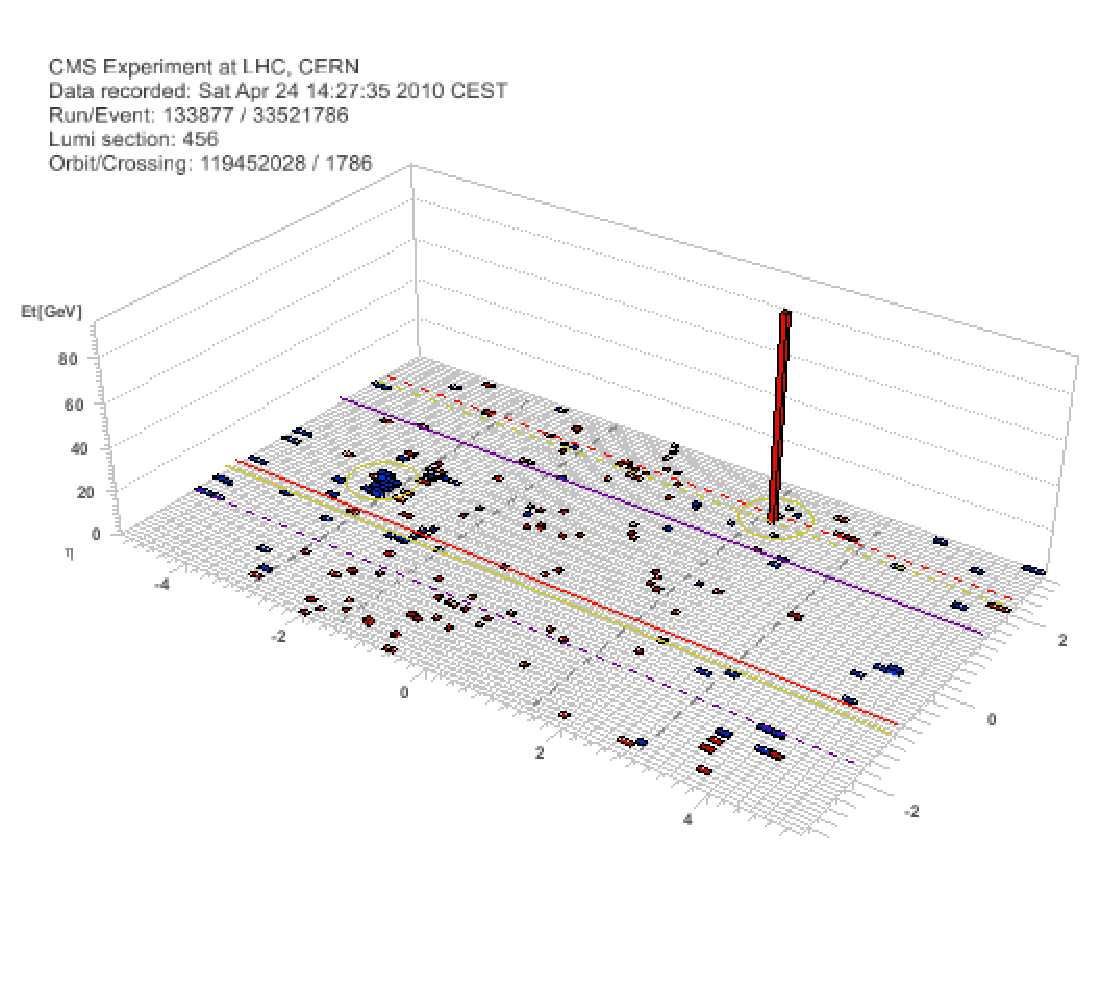
\includegraphics[width=0.47\textwidth]{fig/EEspike.eps} \\
 \end{tabular}
\caption{Example of EB spike (left) and EE spike (right) event}
\label{fig:EBEEspike}
\end{figure}


\subsection{HF, multi-PMT-hits or phi-strip events}
These events are characterized by several PMT hits in adjecent cells; sometimes they show up as
a strip of hits at the same $i\phi$ location, as the ones reported in Figure~\ref{fig:HFmultiHits}. 
This type of noise cannot be cleaned by the existing topological algorithms but could 
be cleaned by the timing or pulse shape based 
cleaning if hits are out-of-time or have a malformed pulse shape. 
A topological cleaning based on the multiplicity of hits above certain energy threshold 
at the same $i\phi$ location might be effective at identifying such noise.
The source of such events is not yet fully understood.

Some of these events are identified by PF cleaning but not by calotower based cleaning.
Studies are ongoing to understand the differences.

%
\begin{figure}[h]
 \centering
 \begin{tabular}{ll}
   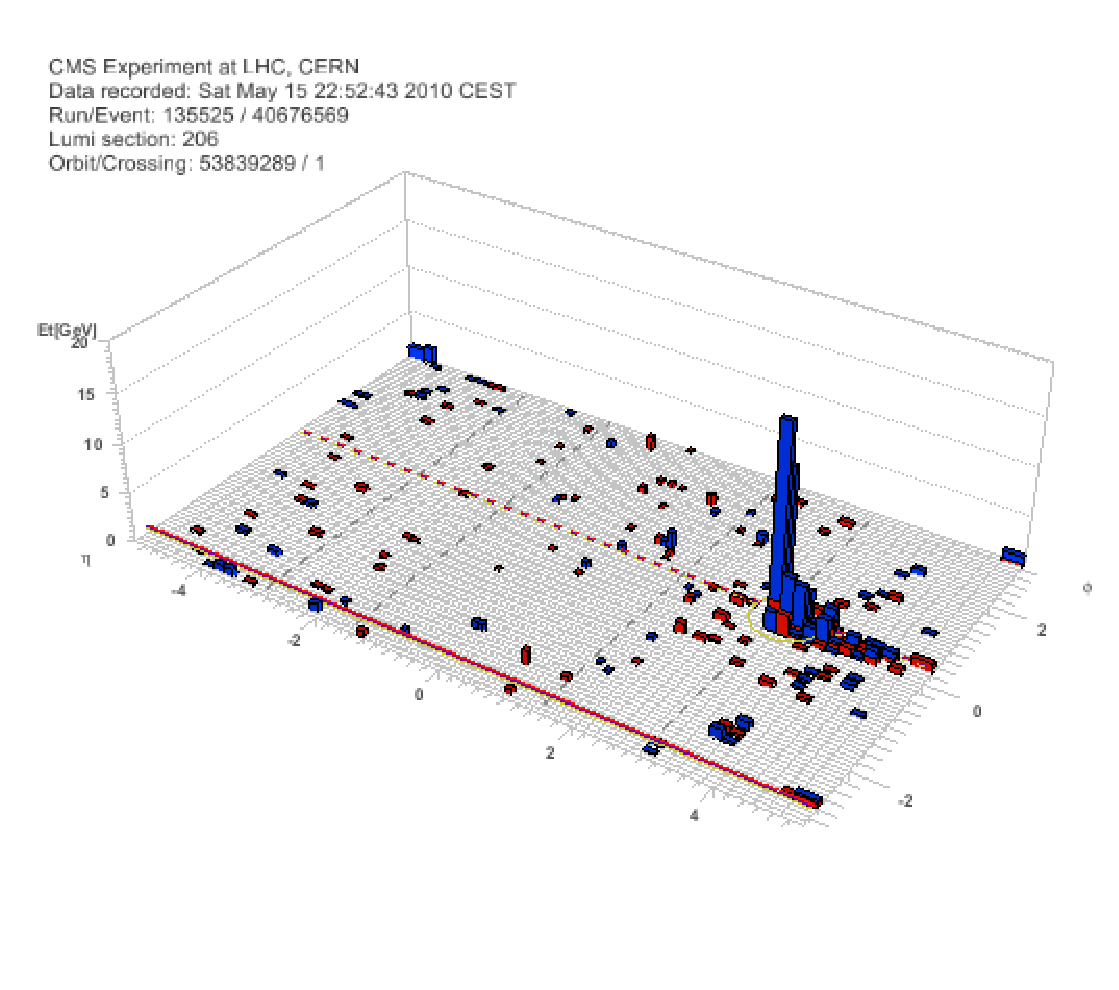
\includegraphics[width=0.47\textwidth]{fig/HFmultiHits.eps} &
   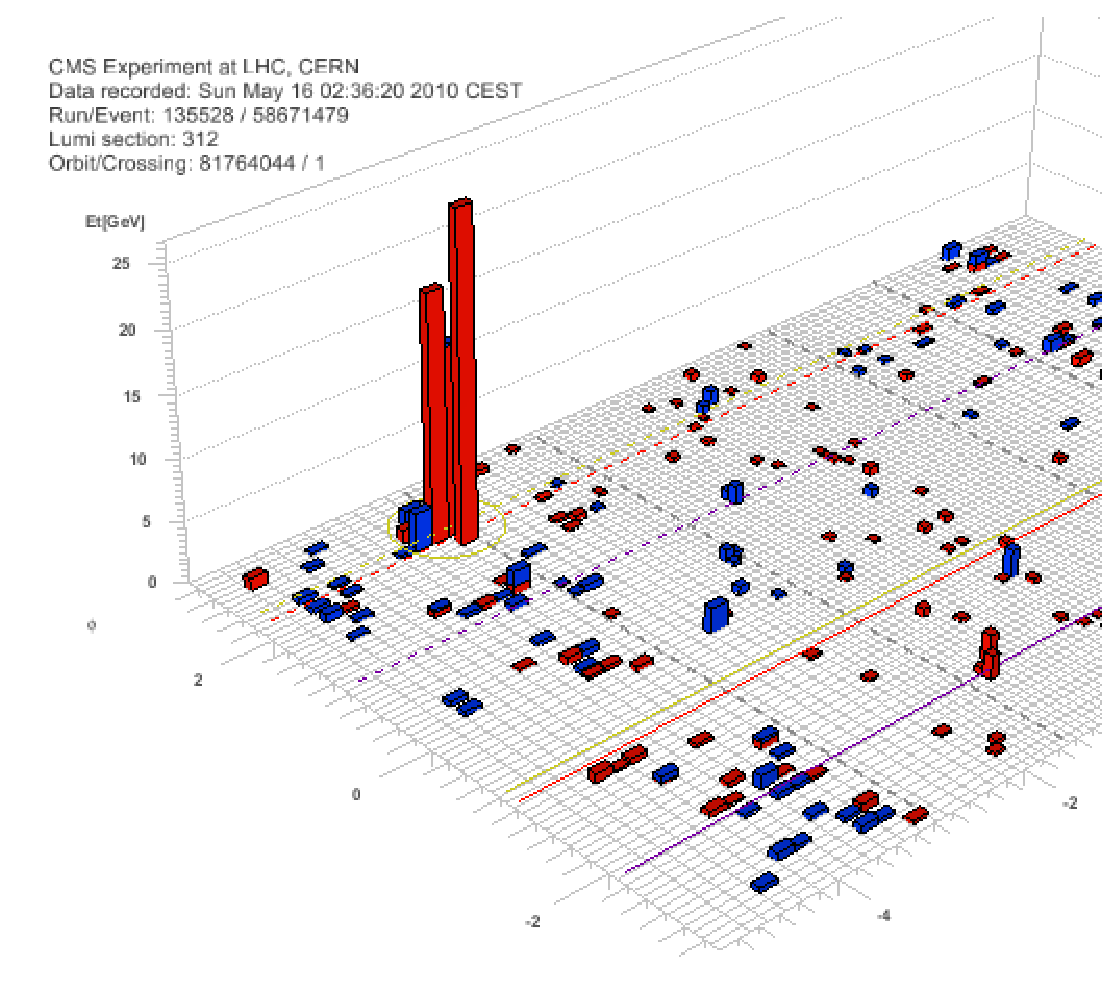
\includegraphics[width=0.47\textwidth]{fig/HFmultiHits_2.eps} \\
 \end{tabular}
\caption{Example of two ``HF multi-PMT-hits or phi-strip'' events}
\label{fig:HFmultiHits}
\end{figure}

\subsection{HF, double-PMT-hits}
These events are characterized by significant energy in both long and short fibers in a single
isolated tower, as shown in Figure~\ref{fig:HFdoublehits}. For high $\etmiss$ events, 
this noise often shows up in the towers located at the smallest $\eta$ 
value in HF ($\eta$=3). This can be explained by the fact that, for a given energy, 
a noise occurring at smaller $\eta$ produces a larger transverse energy, and therefore is more visible at high $\etmiss$.
Anyway it's not excluded that double-hits occurrs also at larger $\eta$; but in this case such events might 
fall in the bulk of $\etmiss$ distribution.

This type of noise cannot be cleaned by current calotower-based topological algorithms (PET or S9/S1) but can
be cleaned by the timing or pulse shape based cleaning if hits are out-of-time or have a malformed pulse shape.
However, cases of in-time double-hits with good pulse shape have been observed. In such cases, a cleaning based on
S$8$/S$1$ isolation variable could be effective, where S$8$/S$1$ is defined in a similar way to S$9$/S$1$
with the companion RecHit energy from the same HF tower left out from the sum. 
On the other hand, this type of cleaning is not expected to be fully safe for isolated particles, 
in particular for physically bigger towers at lower $\eta$ values. 
Preliminary studies on the use of S$8$/S$1$ isolation variable have been performed but not yet finalized. 

PF cleaning can flag some of these noisy events. Studies are ongoing to understand the differences.

%
\begin{figure}[h]
 \centering
 \begin{tabular}{ll}
   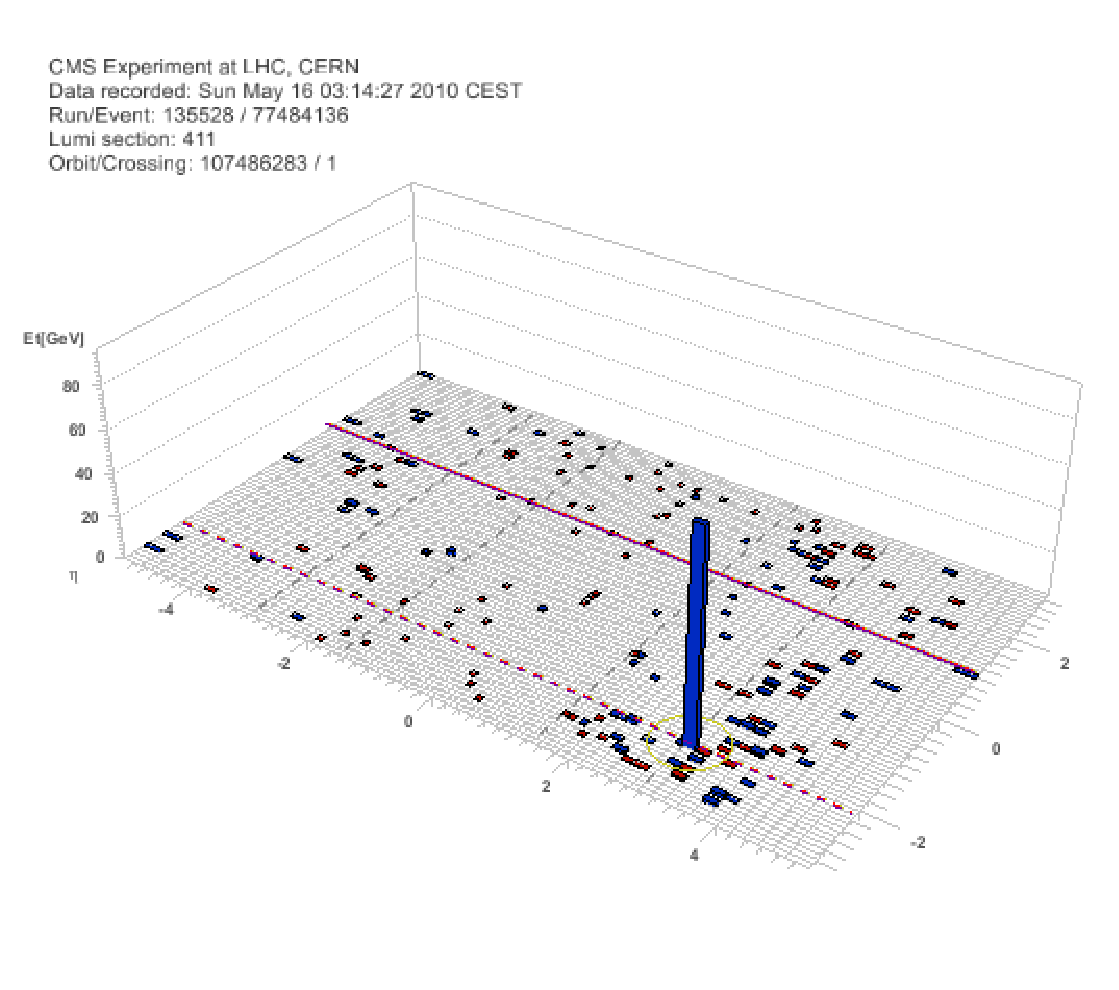
\includegraphics[width=0.47\textwidth]{fig/HFdoubleHit.eps} &
   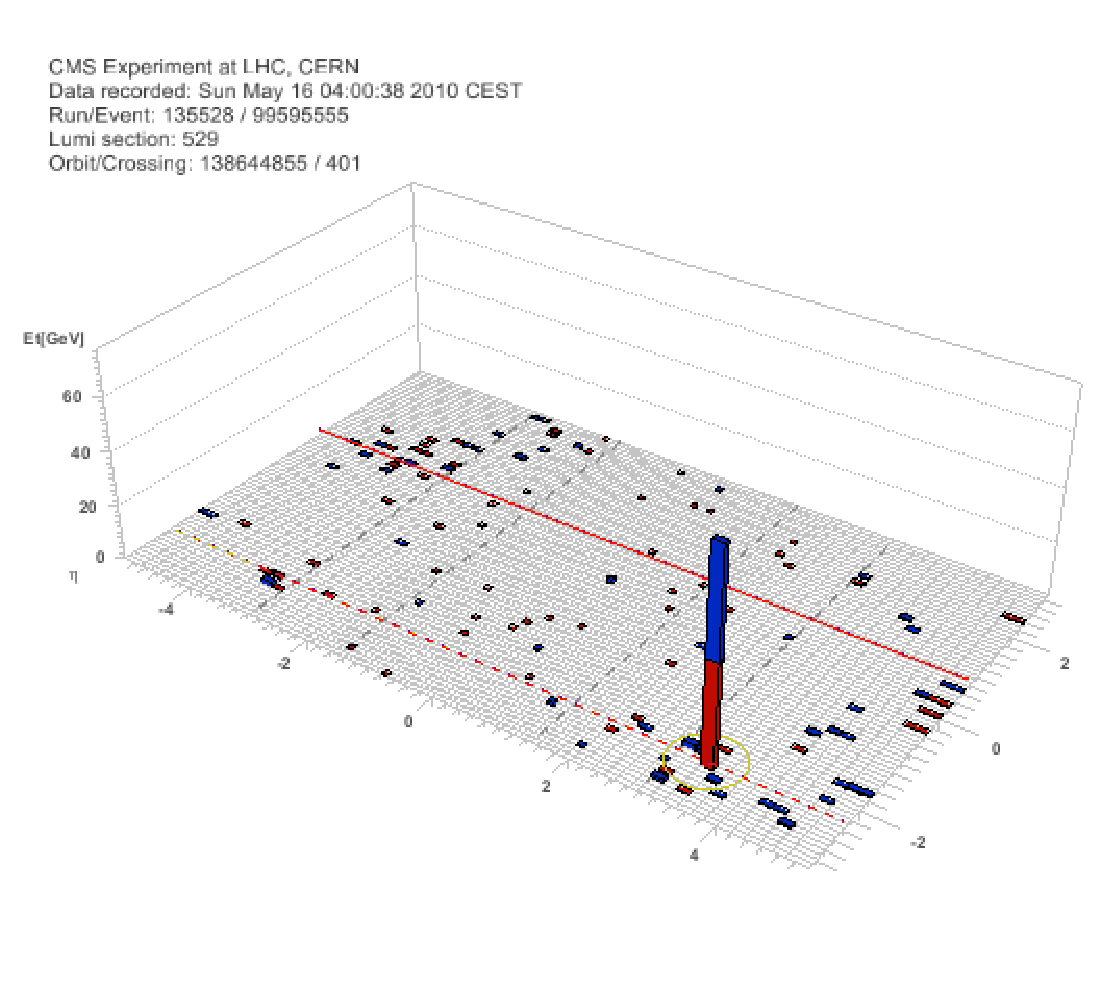
\includegraphics[width=0.47\textwidth]{fig/HFdoubleHit_1.eps} \\
 \end{tabular}
\caption{Example of ``HF double-PMT-hits'' events. Event in left plot is cleaned by PF and not by 
calotower-based cleaning; the event on the right is not cleaned by any of the two. 
NOTE: The event display for the left plot is mis-leading since the hit is not single, 
as it would seems, but double. In fact, in HF, blue=2*$E_{S}$=hadEnergy, while red=$E_{L}-E_{S}$=emEnergy. 
In this event the emEnergy (``red'') is negative, but both energies in long and short fibers, $E_{L}$ and $E_{S}$, are large
(several undreds of GeV). The event display only shows positive quantities 
(only the hadEnergy = ``blue'') so the negative ``red'' is not visible and gives the illusion of a single hit. 
Most of events cleaned by PF have negative emEnergy.}
\label{fig:HFdoublehits}
\end{figure}

\subsection{HF, PMT hit embedded in a jet} ~\label{sec:HFHitEmbeddedInJet}
These events are characterized by one or more anomalous hits embedded inside a jet,as shown in 
Figure~\ref{fig:HFhitEmbeddedInJet}. This type of noise could arise from muons coming from 
in-flight decays of hadronic particles or from a jet punch-through. In both cases
such jets could be identified using the JetID variables since it is expected that a large fraction of the
total jet energy would come from only one or two HF towers. Due to an overlap between real and anomalous signal there are
two cleaning strategies possible: an entire event could be rejected or a more sophisticated anomalous energy
subtraction algorithm would have to be developed.
%
\begin{figure}[h]
 \centering
 \begin{tabular}{ll}
   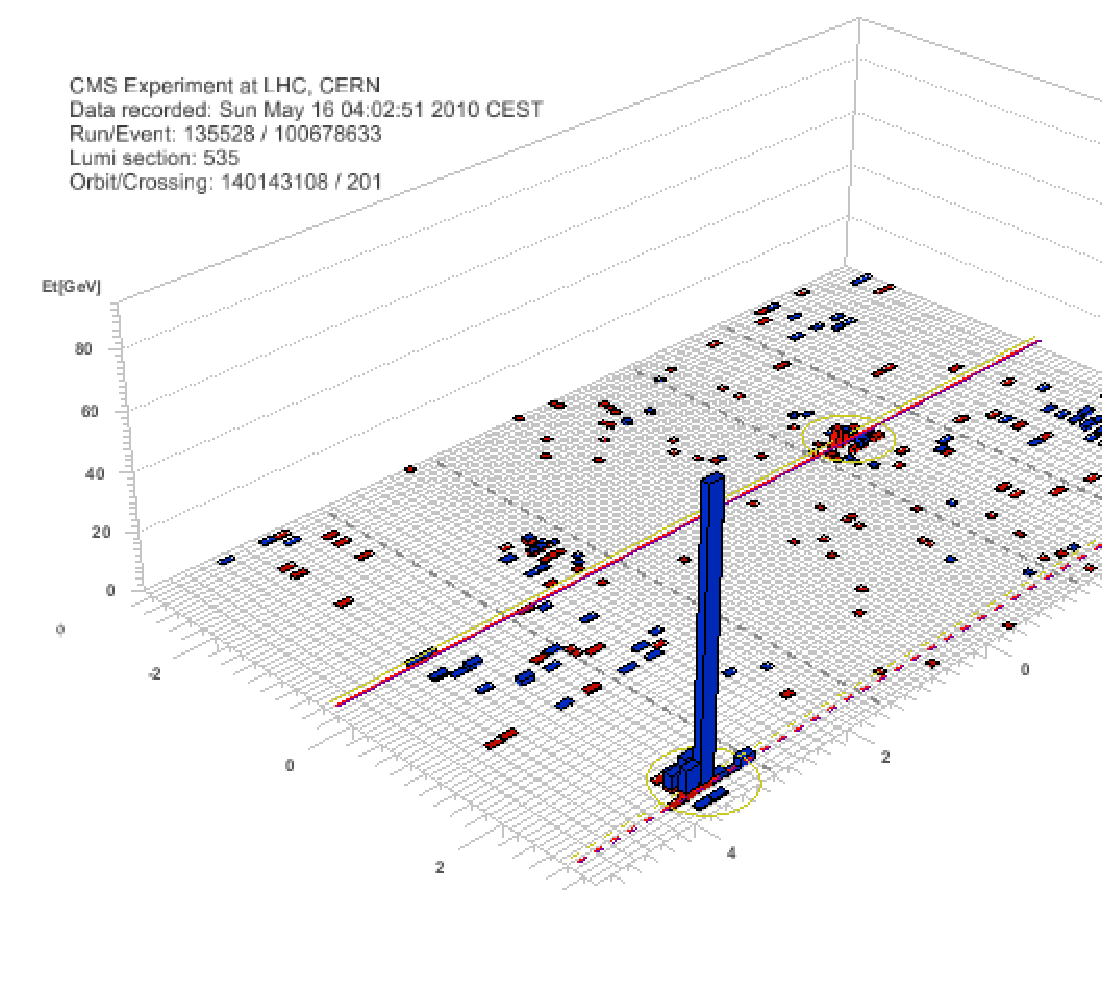
\includegraphics[width=0.47\textwidth]{fig//HFhitInJet.eps} & 
   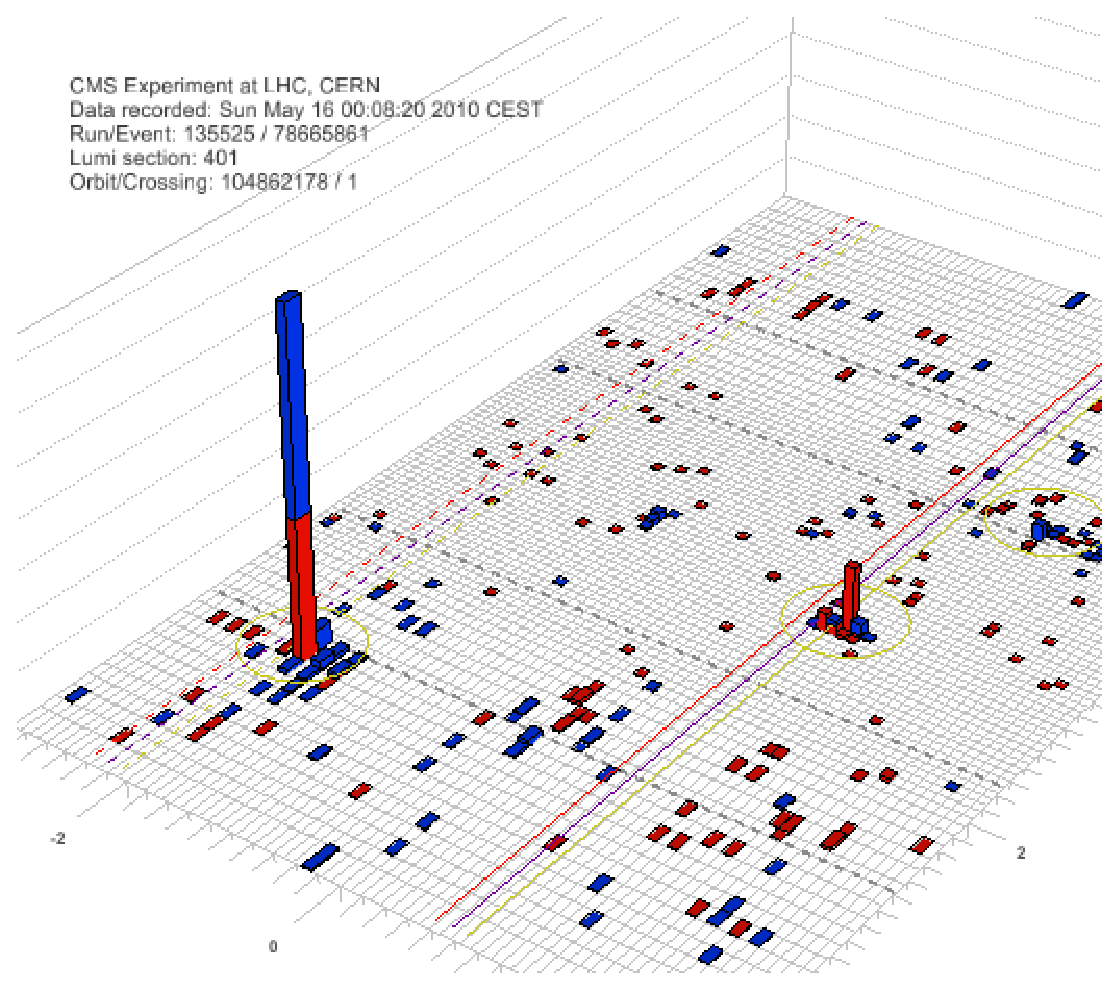
\includegraphics[width=0.47\textwidth]{fig//HFhitInJet_1.eps} \\
 \end{tabular}
\caption{Example of ``HF PMT hit embedded in a jet'' events}
\label{fig:HFhitEmbeddedInJet}
\end{figure}


\clearpage
\section{List of high $\etmiss$ events}

In this section, the complete list of high $\etmiss$ events is provided, for both tc$\etmiss$ 
(Table~\ref{tab:tcMETlist1}, ~\ref{tab:tcMETlist2}, ~\ref{tab:tcMETlist3} ) and pf$\etmiss$ 
(Table~\ref{tab:pfMETlist1}) skims.


% tcMET list Part 1
\begin{table}[htbp]
  \begin{center}
    \begin{tabular}{|c|c|c|c|c|}
      \hline
      Run & Event & LS & tc$\etmiss$ & category \\     
      \hline
      132599 & 4345895     & 183  &    78.2843  & HF multi-PMT-hits or phi-strip events (tcMET $\approx$ pfMET) \\
      132601 & 166842      & 7    &    81.8343  & HF double-PMT-hits  (small pfMET) \\
      132601 & 4585263     & 188  &    237.387  & EB spike at EB-EE boundary (small pfMET) \\
      132658 & 892391      & 37   &    68.8251  & Others, noise in both HB and HE (2 ``jets'' with EMF=0) (small pfMET) \\
      133046 & 3187891     & 138  &    148.51   & EB spike at EB-EE boundary (small pfMET) \\
      133321 & 14516033    & 238  &    60.4839  & HF double-PMT-hits  (small pfMET) \\
      133874 & 41569953    & 528  &    81.4559  & HE noise (tcMET $\approx$ pfMET) \\
      133874 & 66583217    & 826  &    85.6937  & HF double-PMT-hits  (tcMET $\approx$ pfMET) \\
      133877 & 21558793    & 299  &    83.5564  & HF double-PMT-hits  (small pfMET) \\
      133877 & 33521786    & 456  &    90.3345  & EE spike (small pfMET) \\
      133877 & 83377798    & 1130 &    63.9341  & HF double-PMT-hits  (tcMET $\approx$ pfMET) \\
      133885 & 335989      & 5    &    62.133   & Physics 3 jets (1 ``jet'' is an electron of 25~GeV) (tcMET $\approx$ pfMET) \\
      133927 & 369683      & 6    &    93.0333  & HF double-PMT-hits  (small pfMET) \\
      133928 & 22682366    & 319  &    63.7869  & HF multi-PMT-hits or phi-strip events (tcMET $\approx$ pfMET) \\
      133928 & 36620099    & 517  &    66.8677  & Physics 1 jet (in endcap) (tcMET $\approx$ pfMET) \\
      135149 & 63603939    & 753  &    66.9592  & Physics 2 jets (2 electrons of 7 and 3 GeV) (small pfMET=15.9 GeV) \\
      135149 & 116927949   & 1265 &    63.1608  & Physics 3 jets (low $p_T$ electrons) (tcMET $\approx$ pfMET) \\
      135149 & 154572404   & 1625 &    98.3469  & Physics 3 jets (low $p_T$ electrons) (tcMET $\approx$ pfMET) \\
      135149 & 155186256   & 1631 &    60.8672  & Physics 3 jets (20 GeV muon) (tcMET $\approx$ pfMET) \\
      135149 & 156347129   & 1642 &    65.4799  & HF double-PMT-hits (small pfMET) \\
      135149 & 162208514   & 1699 &    78.278   & HF multi-PMT-hits or phi-strip events (tcMET $\approx$ pfMET) \\ 
      135149 & 214116071   & 2215 &    66.5431  & HF PMT hit embedded in a jet (tcMET $\approx$ pfMET) \\
      135149 & 215931499   & 2233 &    71.0733  & Physics 4 jets (27 GeV electron) (tcMET $\approx$ pfMET) \\
      135149 & 217153658   & 2245 &    81.4574  & Physics 3 jets (26 GeV and 6 GeV muons)(tcMET $\approx$ pfMET) \\
      135149 & 222730662   & 2307 &    418.801  & EB spike at EB-EE boundary (small pfMET) \\ 
      135149 & 233103931   & 2411 &    74.2742  & EB spike at EB-EE boundary (small pfMET) \\ 
      135149 & 267019811   & 2758 &    66.3561  & Physics 4 jets (low $p_T$ electron)(small pfMET=19.8 GeV) \\
      135149 & 318396401   & 3297 &    542.981  & EB spike at EB-EE boundary (small pfMET) \\
      135175  & 17812005     & 191  &    64.2943 & HB noise (tcMET $\approx$ pfMET) \\
      135175  & 42757899     & 426  &    92.0741 & HF double-PMT-hits (small pfMET) \\
      135175  & 46362317     & 460  &    69.9842 & Physics 6 jets (tcMET ~ 2 * pfMET) \\
      135175  & 57982991     & 574  &    73.1318 & HF double-PMT-hits (small pfMET) \\
      \hline
    \end{tabular}
    \caption{List of events with tc$\etmiss>60$~GeV - Part 1.}        
    \label{tab:tcMETlist1}
  \end{center}
\end{table}


% tcMET list Part 2
\begin{table}[htbp]
  \begin{center}
    \begin{tabular}{|c|c|c|c|c|}
      \hline
      Run & Event & LS & tc$\etmiss$ & category \\     
      \hline
      135175  & 64940222     & 641  &    62.4991 & EB spike at EB-EE boundary (small pfMET) \\
      135175  & 72861680     & 718  &    116.591 & EE spike (small pfMET) \\
      135175  & 94014613     & 926  &    145.352 & Physics 4 jets (low $p_T$ electrons) (tcMET ~ 2 * pfMET) \\
      135175  & 100575970    & 990  &    61.3085 & HF double-PMT-hits (tcMET $\approx$ pfMET) \\
      135521  & 22453149     & 203  &    71.9826 & Physics 3 jets (18 GeV electron)(tcMET $\approx$ pfMET) \\
      135521  & 32219215     & 251  &    69.445  & Physics 2 jets (both in HF) (tcMET $\approx$ pfMET) \\
      135521  & 40089571     & 289  &    77.7739 & EB spike at EB-EE boundary (small pfMET) \\
      135521  & 66824775     & 420  &    80.9651 & EB spike at EB-EE boundary (small pfMET) \\
      135521  & 69919879     & 435  &    80.0659 & HF multi-PMT-hits or phi-strip events (small pfMET), eta strip \\
      135523  & 9879701      & 50   &    61.4423 & HF double-PMT-hits (small pfMET) \\
      135523  & 16543369     & 84   &    164.131 & HB noise (tcMET $\approx$ pfMET) \\
      135523  & 28853462     & 145  &    64.5248 & Physics 2 jets (4.5 GeV muon) (tcMET $\approx$ pfMET) \\
      135525  & 17433547     & 87   &    68.2453 & Physics 3 jets (small pfMET = 7 GeV) \\ 
      135525  & 40676569     & 206  &    62.4033 & HF multi-PMT-hits or phi-strip events (tcMET $\approx$ pfMET), 2-4 phi strip \\
      135525  & 45035068     & 228  &    70.4362 & EB spike at EB-EE boundary (small pfMET) \\
      135525  & 48804509     & 247  &    62.6639 & Physics 4 jets (tcMET $\approx$ pfMET) \\
      135525  & 63386076     & 320  &    77.1017 & HF multi-PMT-hits or phi-strip events (tcMET $\approx$ pfMET) \\
      135525  & 78665861     & 401  &    62.0925 & HF PMT hit embedded in a jet (tcMET $\approx$ pfMET) \\
      135525  & 80550953     & 410  &    65.2472 & Physics 2 jets (back-to-back) (tcMET ~ 2 * pfMET) \\
      135525  & 87558102     & 448  &    110.215 & Physics 5 jets (tcMET $\approx$ pfMET) \\ 
      135525  & 88031668     & 450  &    64.1569 & Physics 4 jets (tcMET ~ 3 * pfMET) \\
      135528  & 884119       & 5    &    62.3458 & HF double-PMT-hits (tcMET $\approx$ pfMET) \\
      135528  & 19813983     & 105  &    61.8938 & HF multi-PMT-hits or phi-strip events (tcMET $\approx$ pfMET) \\
      135528  & 32603499     & 174  &    63.8757 & EB spike at EB-EE boundary (small pfMET) \\
      135528  & 58671479     & 312  &    64.5086 & HF multi-PMT-hits or phi-strip events (small pfMET) \\
      135528  & 60003196     & 319  &    74.3878 & Physics 2 jets (back-to-back) (small pfMET = 17 GeV) \\
      135528  & 77484136     & 411  &    89.8829 & HF double-PMT-hits (small pfMET) \\
      135528  & 80490418     & 426  &    73.026  & Physics 3 jets (8 GeV muon) (tcMET ~ 2 * pfMET) \\
      135528  & 99595555     & 529  &    82.2867 & HF double-PMT-hits (tcMET $\approx$ pfMET) \\
      135528  & 100678633    & 535  &    78.523  & HF PMT hit embedded in a jet (tcMET $\approx$ pfMET) \\
      135528  & 102808626    & 546  &    68.4343 & Physics 6 jets (6 GeV electron) (tcMET ~ 2 * pfMET) \\
      135528  & 115447830    & 618  &    62.2738 & HB noise (tcMET $\approx$ pfMET) \\
      135528  & 130731462    & 699  &    127.18  & HF double-PMT-hits (small pfMET) \\
      \hline
    \end{tabular}
    \caption{List of events with tc$\etmiss>60$~GeV - Part 2.}        
    \label{tab:tcMETlist2}
  \end{center}
\end{table}


% tcMET list Part 3
\begin{table}[htbp]
  \begin{center}
    \begin{tabular}{|c|c|c|c|c|}
      \hline
      Run & Event & LS & tc$\etmiss$ & category \\     
      \hline
      135528  & 150342996    & 808  &    66.7701 & Physics 5 jets (tcMET ~ 2 * pfMET) \\
      135528  & 153336127    & 824  &    63.8531 & Physics 4 jets (28.5 and 14 GeV electrons) (tcMET $\approx$ pfMET) \\
      135528  & 162079374    & 871  &    111.931 & HF multi-PMT-hits or phi-strip events (small pfMET) \\
      135528  & 172155075    & 927  &    216.754 & EB spike at EB-EE boundary (small pfMET) \\
      135528  & 178385490    & 960  &    113.215 & HF multi-PMT-hits or phi-strip events (small pfMET) \\
      135528  & 194937806    & 1049 &    61.32   & Physics 4 jets (10 GeV electron) (tcMET $\approx$ pfMET) \\
      135528  & 195017684    & 1050 &    65.1985 & HF double-PMT-hits (small pfMET) \\
      135528  & 204463628    & 1103 &    69.0627 & Physics 2 jets (small pfMET =  14 GeV) \\
      135528  & 207348623    & 1118 &    75.5706 & HF multi-PMT-hits or phi-strip events (tcMET $\approx$ pfMET) \\ 
      135528  & 215351211    & 1162 &    68.9099 & EB spike at EB-EE boundary (small pfMET) \\
      135528  & 226804792    & 1227 &    575.609 & EB spike at EB-EE boundary (small pfMET) \\
      135528  & 227722743    & 1232 &    159.545 & EB spike at EB-EE boundary (small pfMET) \\
      135528  & 238836923    & 1292 &    69.2778 & EB spike at EB-EE boundary (small pfMET) \\
      135528  & 256160509    & 1388 &    74.4981 & EB spike at EB-EE boundary (small pfMET) \\
      135535  & 15564358     & 92   &    224.509 & HB noise (tcMET $\approx$ pfMET) \\
      135535  & 18401448     & 109  &    79.3533 & HF double-PMT-hits (small pfMET) \\
      135535  & 31027189     & 182  &    67.2768 & Others - HB activity + muon (tcMET $\approx$ pfMET) \\
      135573  & 13003948     & 151  &    81.3199 & HF double-PMT-hits (small pfMET) \\
      135575  & 5342229      & 38   &    63.8363 & Physics 3 jets (2 GeV muon) (tcMET ~ 2 * pfMET) \\
      135575  & 11156890     & 79   &    61.2564 & Physics 3 jets (6 GeV muon) (tcMET $\approx$ pfMET) \\
      135575  & 13695733     & 97   &    235.509 & EB spike at EB-EE boundary (small pfMET) \\
      135575  & 64338278     & 393  &    68.2189 & Physics 2 jets (1 jet at barrel-endcap border)(tcMET $\approx$ pfMET) \\
      135575  & 67135767     & 408  &    68.972  & HF multi-PMT-hits or phi-strip events (small pfMET) \\
      135575  & 67221216     & 409  &    78.3203 & EB spike at EB-EE boundary (small pfMET) \\
      135575  & 69788619     & 423  &    63.2861 & Physics 4 jets (27 and 10 GeV electrons) (tcMET $\approx$ pfMET) \\
      135575  & 93340831     & 559  &    146.205 & Physics 2 jets + 65 GeV muon in jet + EB activity at border? (tcMET $\approx$ pfMET) \\
      135575  & 96504815     & 577  &    60.6013 & EB spike at EB-EE boundary (small pfMET) \\
      135575  & 117083855    & 698  &    86.9326 & HF double-PMT-hits (small pfMET) \\
      135575  & 126932629    & 757  &    72.2135 & HF double-PMT-hits (small pfMET) \\
      135575  & 128277130    & 765  &    64.6596 & Physics 3 jets (tcMET ~ 2 * pfMET) \\
      135575  & 129789830    & 774  &    66.7404 & HB noise (tcMET $\approx$ pfMET), Ion Feedback? \\
      135575  & 130735782    & 779  &    64.1565 & EB spike at EB-EE boundary (small pfMET) \\
      135575  & 134419161    & 805  &    61.4918 & HF PMT hit embedded in a jet (small pfMET) \\
      135575  & 144805158    & 870  &    86.8711 & HF double-PMT-hits (small pfMET) \\
      135575  & 149874280    & 901  &    61.6245 & EB spike at EB-EE boundary (small pfMET) \\
      135575  & 180503581    & 1110 &    64.2686 & HF double-PMT-hits (small pfMET) \\
      135575  & 189427985    & 1175 &    61.6306 & Physics 2 jets (23, and 2 GeV electrons)(tcMET ~ 2 * pfMET) \\
      135575  & 190898956    & 1186 &    73.6522 & EB spike at EB-EE boundary (small pfMET) \\
      135575  & 192395010    & 1197 &    64.455  & Physics 3 jets (tcMET ~ 2 * pfMET) \\
      135575  & 193746493    & 1207 &    104.321 & HB noise (tcMET $\approx$ pfMET) \\
      135735  & 8376298      & 103  &    72.7973 & Physics 4 jets (2.6 GeV electron) (small pfMET=18 GeV) \\
      135735  & 22883658     & 169  &    83.7303 & EB spike (small pfMET) \\       
      \hline
    \end{tabular}
    \caption{List of events with tc$\etmiss>60$~GeV - Part 3.}        
    \label{tab:tcMETlist3}
  \end{center}
\end{table}



% pfMET list Part 1
\begin{table}[htbp]
  \begin{center}
    \begin{tabular}{|c|c|c|c|c|}
      \hline
      Run & Event & LS & pf$\etmiss$ & category \\     
      \hline
      132599 & 4345895     &  183  &    67.483   & HF multi-PMT-hits or phi-strip events (pfMET $\approx$ tcMET) \\ 
      133874 & 41569953    &  528  &    85.4173  & HE noise (pfMET $\approx$ tcMET) \\
      133874 & 66583217    &  826  &    94.6307  & HF double-PMT-hits  (pfMET $\approx$ tcMET) \\
      133877 & 9967629     &  147  &    63.2921  & Physics 2 jets (pfMET $\approx$ tcMET) \\
      133877 & 83377798    &  1130 &    62.5759  & HF double-PMT-hits  (pfMET $\approx$ tcMET) \\
      133885 & 335989      &  5    &    65.6229  & Physics 3 jets (1 ``jet'' is an electron of 25~GeV) (pfMET $\approx$ tcMET) \\ 
      133928 & 36620099    &  517  &    67.8891  & Physics 1 jet (in endcap) (pfMET $\approx$ tcMET) \\ 
      135149 & 116927949   &  1265 &    72.6891  & Physics 3 jets (low $p_T$ electrons) (pfMET $\approx$ tcMET) \\ 
      135149 & 122427147   &  1317 &    528.658  & Others large muon-induced pfMET, very small caloMET/tcMET \\
      135149 & 154572404   &  1625 &    63.0696  & Physics 3 jets (low $p_T$ electrons) (pfMET $\approx$ tcMET) \\ 
      135149 & 162208514   &  1699 &    70.1507  & HF multi-PMT-hits or phi-strip events (pfMET $\approx$ tcMET) \\
      135149 & 215931499   &  2233 &    86.0465  & Physics 4 jets (27 GeV electron) (pfMET $\approx$ tcMET) \\ 
      135149 & 217153658   &  2245 &    67.7884  & Physics 3 jets (26 GeV and 6 GeV muons)(pfMET $\approx$ tcMET) \\ 
      135175 & 57397642    &  568  &    337.561  & Others large muon-induced pfMET, very small caloMET/tcMET \\
      135175 & 94014613    &  926  &    61.3586  & Physics 4 jets (low $p_T$ electrons) (tcMET ~ 2 * pfMET) \\ 
      135175 & 100575970   &  990  &    61.8675  & HF double-PMT-hits (pfMET $\approx$ tcMET) \\
      135521 & 22774568    &  205  &    60.8714  & Physics 3 jets (pfMET $\approx$ tcMET) \\
      135521 & 32219215    &  251  &    62.8553  & Physics 2 jets (both in HF) (pfMET $\approx$ tcMET) \\ 
      135523 & 16543369    &  84   &    179.233  & HB noise (pfMET $\approx$ tcMET) \\
      135525 & 48804509    &  247  &    60.366   & Physics 4 jets (pfMET $\approx$ tcMET) \\
      135525 & 63386076    &  320  &    67.772   & HF multi-PMT-hits or phi-strip events (pfMET $\approx$ tcMET) \\
      135525 & 78665861    &  401  &    62.6467  & HF PMT hit embedded in a jet (pfMET $\approx$ tcMET) \\
      135525 & 87558102    &  448  &    121.168  & Physics 5 jets (pfMET $\approx$ tcMET) \\
      135528 & 32056404    &  171  &    231.068  & Others large muon-induced pfMET, very small caloMET/tcMET \\
      135528 & 99411269    &  528  &    62.2593  & HB noise (pfMET $\approx$ tcMET) , Ion Feedback? \\
      135528 & 99595555    &  529  &    80.0732  & HF double-PMT-hits (pfMET $\approx$ tcMET) \\
      135528 & 99860976    &  531  &    69.2713  & Physics 6 jets (pfMET ~ 2*tcMET) \\
      135528 & 100678633   &  535  &    67.2221  & HF PMT hit embedded in a jet (pfMET $\approx$ tcMET) \\
      135528 & 109847963   &  584  &    83.8501  & Others large muon-induced pfMET, very small caloMET/tcMET \\
      135528 & 115447830   &  618  &    72.7202  & HB noise (pfMET $\approx$ tcMET) \\
      135528 & 190129212   &  1023 &    64.6779  & Physics 2 jets + muon (pfMET $\approx$ tcMET) \\
      135528 & 192636869   &  1037 &    66.284   & HF PMT hit embedded in a jet (pfMET ~ 2 * tcMET) \\
      135528 & 207348623   &  1118 &    68.2922  & HF multi-PMT-hits or phi-strip events (pfMET $\approx$ tcMET) \\
      135528 & 208274999   &  1123 &    60.6407  & Others large muon-induced pfMET, very small caloMET/tcMET \\
      135535 & 15564358    &  92   &    235.597  & HB noise (pfMET $\approx$ tcMET) \\
      135535 & 31027189    &  182  &    72.7387  & Others - HB activity + muon (pfMET $\approx$ tcMET) \\
      135575 & 11156890    &  79   &    66.5948  & Physics 3 jets (6 GeV muon) (pfMET $\approx$ tcMET) \\ 
      135575 & 64338278    &  393  &    64.4694  & Physics 2 jets (1 jet at barrel-endcap border)(pfMET $\approx$ tcMET) \\ 
      135575 & 75318623    &  455  &    60.9222  & Physics jet + muon (pfMET $\approx$ tcMET) \\
      135575 & 93340831    &  559  &    152.727  & Physics 2 jets + 65 GeV muon in jet + EB activity at border? (pfMET $\approx$ tcMET) \\ 
      135575 & 129789830   &  774  &    76.5243  & HB noise (pfMET $\approx$ tcMET) , Ion Feedback? \\
      135575 & 136780600   &  820  &    64.009   & HB noise (pfMET $\approx$ tcMET) , Ion Feedback? \\
      135575 & 193746493   &  1207 &    112.707  & HB noise (pfMET $\approx$ tcMET) \\
      \hline
    \end{tabular}
    \caption{List of events with pf$\etmiss>60$~GeV.}        
    \label{tab:pfMETlist1}
  \end{center}
\end{table}

\clearpage
\section{Conclusions}
We presented a study of the performance of raw calorimetric $\etmiss$
reconstruction in proton-proton collision events collected by the CMS
experiment during the LHC commissioning phase in December 2009. Data
samples collected at $\sqrt{s}=900$ and $2360$~GeV are analyzed in this
note. Comparisons of $\etmiss$ and related quantities in collision data
with Monte Carlo simulation showed a good agreement. It was observed
that the collision energy in the forward region is modeled
reasonably well, and $\etmiss$ resolutions are in decent agreement with
simulation. A set of HCAL and ECAL noise clean up algorithms was implemented, and
these algorithms perform quite well in the MinBias dataset. A few events that
remain in $\etmiss$ tails seem to originate from HCAL noise. More
sophisticated algorithms for identifying anomalous noise 
events in HCAL and ECAL will need to be developed.

\input{Bib}

\end{linenumbers}
\end{document}

